\documentclass[a4paper]{article}

%% Language and font encodings
\usepackage[brazil,english]{babel}
\usepackage[utf8x]{inputenc}
\usepackage[T1]{fontenc}
\usepackage{listings}
\usepackage{amsmath}
\lstset{backgroundcolor=\color{mygray}}
\usepackage{float}
\usepackage{amsfonts}
\selectlanguage{brazil}
%% Package for Matlab input
\usepackage{color} %red, green, blue, yellow, cyan, magenta, black, white
\definecolor{mygreen}{RGB}{28,172,0} % color values Red, Green, Blue
\definecolor{mylilas}{RGB}{170,55,241}
\definecolor{mygray}{RGB}{245,245,245}
\lstset{language=Matlab,%
    %basicstyle=\color{red},
    breaklines=true,%
    morekeywords={matlab2tikz},
    keywordstyle=\color{blue},
    morekeywords=[2]{1}, keywordstyle=[2]{\color{black}},
    identifierstyle=\color{black},
    stringstyle=\color{mylilas},
    commentstyle=\color{mygreen},
    showstringspaces=false,%without this there will be a symbol in the places where there is a space
    numbers=left,
    numberstyle={\tiny \color{black}},% size of the numbers
    numbersep=9pt, % this defines how far the numbers are from the text
    emph=[1]{for,end,break},emphstyle=[1]\color{red}, %some words to emphasise
    emph=[2]{word1,word2}, emphstyle=[2]{style}} 
%% Sets page size and margins
\usepackage[a4paper,top=3cm,bottom=2cm,left=3cm,right=3cm,marginparwidth=1.75cm]{geometry}
%% Useful packages
\usepackage{amsmath}
\usepackage{graphicx} %% adiciona imagem
\usepackage[colorinlistoftodos]{todonotes}
\usepackage[colorlinks=true, allcolors=blue]{hyperref}
\usepackage{subcaption}

\title{Notas de Aula de Labortório de curvas e superfícies}
\author{Asla Medeiros e Sá e alunos da turma 2017}

\begin{document}
\maketitle 

\section{Introdução}

A visualização dos conceitos formalizados em geometria diferencial 
podem ser de grande auxílio didático e também para a dar suporte "concreto" à intuição geométrica de conceitos como curvatura e torção.  O propórito destas notas de aula é o de compilar o material abordado nas aulas de laboratório computacional da disciplina de curvas e superfícies. O intuito é documentar o que foi abordado em laboratório para consulta futura. 

\section{Ambientes gráficos}

Para o desenho de curvas e também de superfícies, se faz necessário lançar mão de ferramentas computacionais especializadas para esta finalidade. Para curvas planas temos a disposição muitas opções. A primeira classe de ferramentas da qual podemos lançar mão são as calculadoras gráficas. Neste caso optamos por explorar o uso da calculadora gráfica Desmos (https://www.desmos.com/). Outra classe de ferramentas são os ambientes de geometria dinâmica, dentre os quais, o Geogebra (https://www.geogebra.org/) é de longe o mais popular. 

Utilizamos tanto o Desmos quanto o Geogebra com a finalidade de explorar conceitos como parametrização de uma curva. Ao passar para a visualização de curvas no espaço, quisemos visualizar os vetores tangente, normal e binormal, para esclarecer a intuição do que vem a ser a curvatura e a torção de uma dada curva no espaço. Neste momento lançamos mão do Geogebra 3D para fazer diversas visualizações.

Ao estudarmos curvas cuja descrição é mais complexa, percebemos a vantagem de se trabalhar em ambientes computacionais que tratam as equações que definem as curvas de forma simbólica. Em tais ambientes, operações como derivação são executadas simbolicamente, proporcionando clareza aos códigos e evitando erros de cálculo e de transcrições de fórmulas, no caso de a derivação ser feita em um ambiente - WolframAlpha por exemplo - e o resultado ser transcrito para um ambietende desenho.

Para o desenho de superfícies o ambiente do Geogebra 3D foi utilizado para os casos mais simples. Uma sugestão interessante de sofware que permite explorar famílias de superfícies de forma eficiente é o k3DSurf (http://k3dsurf.sourceforge.net/). Seguimos então com a abordagem simbólica para produção de desenhos de superfícies em Matlab. 

Passaremos agora a descrever alguns exercícios que foram feitos no decorrer do curso, definindo os conceitos abordados no exercício e mostrando a implementação que foi feita para produção das imagens. 

\section{Curvas Planas}

Aa seguintes curvas possuem o mesmo traço: ${f(x; y) \in R^2 : x^2 + y^2 = 1}$:

\[\alpha(t) = (cos(t); sin(t)); t \in [0, 2];\]

\[\beta(t) = (cos(2t); sin(2t)); t \in [0, 2]\]

No entanto, a velocidade de $\beta$ é o dobro da velocidade de $\alpha$. 
No mesmo período de tempo, a curva $\beta$ percorre duas vezes a circunferência e a curva $\alpha$ só uma vez.
Quando falamos de velocidade, ver a dinâmica do objeto de estudo em movimento é de grande utilidade cognitiva. Pela simplicidade do exemplo proposto, vamos observar a dinamica do movimento inserindo as equações das curvas $\alpha$ e $\beta$ no ambiente da calculadora gráfica Desmos.

\begin{figure}[ht]
\centering
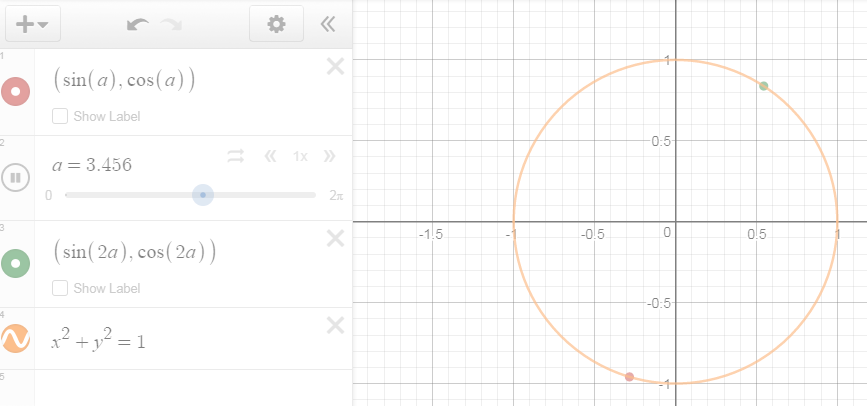
\includegraphics[width=0.7\textwidth]{desmos_circ.png}
\caption{\label{fig:desmos_circ} Exemplo de traço de circunferência no ambiente Desmos.}
\end{figure}

Como parametrizamos um segmento de uma parábola? Fazer desenho.

Como parametrizamos uma circunferência? Mostrar o vetor velocidade.Repetir o exemplo acima no geogebra.


\subsection{Ambiente de geometria dinâmica: Geogebra}

\subsection{Matlab}

\section{Ambiente Simbólico do Matlab}

\section{Curvas no espaço}
\subsection{Geogebra}

\subsection{Matlab}



First you have to upload the image file from your computer using the upload link the project menu.  Figure \ref{fig:curvaEspaco} example.

\begin{figure}[ht]
\centering
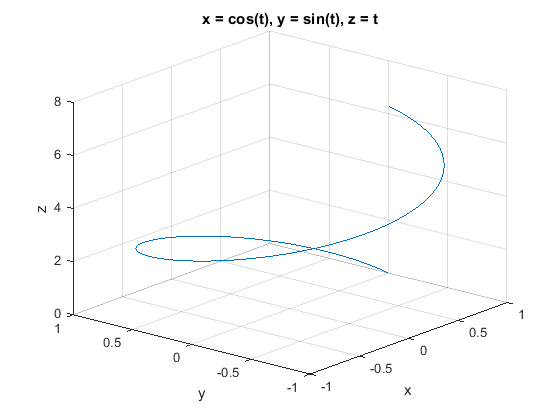
\includegraphics[width=0.7\textwidth]{curvaEspaco.png}
\caption{\label{fig:curvaEspaco} Exemplo de curva no espaço.}
\end{figure}

\subsection{Triedro de Frenet(Rafael Katz)}
As fórmulas de Frenet–Serret descrevem as propriedades cinemáticas de uma partícula que se move ao longo de uma curva contínua e diferenciável,  num espaço euclidiano tridimensional $\mathbb{R^3}$, ou as propriedades geométricas da própria curva independentemente do movimento.

Dada:$\alpha: I \rightarrow \mathbb{R}^3$ parametrizada pelo comprimento de arco sem pontos singulares, definimos o triedro de Frenet como:

\[\{t(s);n(s);b(s)\}\]
Onde t é o vetor unitário  tangente à curva, n é a derivada de t, e  b é o produto vetorial de t e n.


Chamamos de fórmulas de Frenet-Serret o conjunto de equações

\[ \begin{cases}

t'(s) =\kappa(s)n(s),\\

n'(s) =-\kappa(s)t(s) -\tau(s)b(s),\\ 

 b1(s) =\tau(s)n(s)
\end{cases} \]

\begin{figure}[h!]
  \caption{Triedro de Frenet}
  \centering
  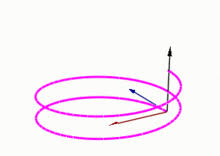
\includegraphics[width=0.5\textwidth]{triedro_frenet.png}
\end{figure}

\subsection{Plano Osculador(Rafael Katz)}
O plano osculatório (gerado por T e N) é um plano em um espaço euclidiano ou espaço afim que atende uma subvariedade em um ponto de forma a ter uma segunda ordem de contato no ponto. A palavra osculate é do osculatus latino que é um particípio passado de osculari, que significa beijar. Um plano osculatório é, portanto, um plano que "beija" uma subvariedade.

O plano osculatório na geometria das curvas espaciais euclidianas pode ser descrito em termos das fórmulas Frenet-Serret como o espaço vectorial gerado dos vetores tangente e normal

\begin{figure}[h!]
  \caption{Plano Osculador}
  \centering
  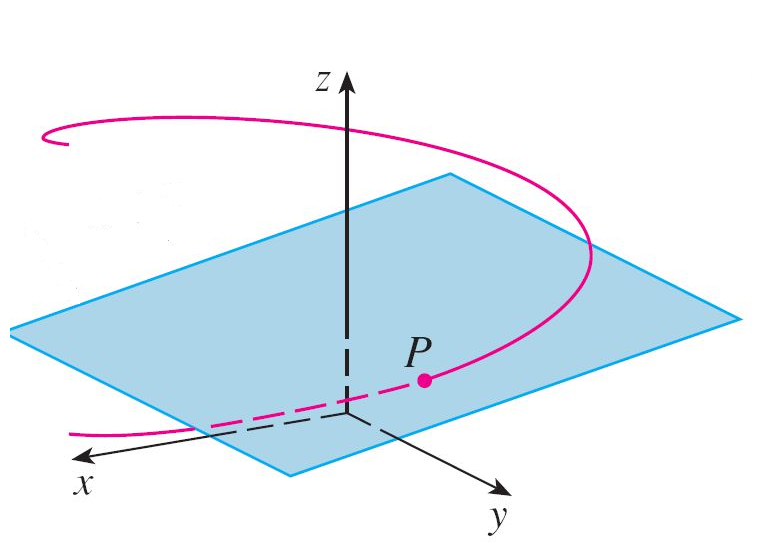
\includegraphics[width=0.5\textwidth]{plano_osculador.png}
\end{figure}

\subsubsection*{Um exemplo de um Plano Osculador feito em Matlab:}

\begin{lstlisting}[frame=single]
syms t;
a = 1;
r = 1;
figure(1);
alpha1 = [t,t^2,t^3];
ezplot3(alpha1(1),alpha1(2),alpha1(3),[0,2*pi,0.01,pi]);
axis([-5 5 -5 5]);
for k = 0:0.1:2
    alpha1 = [t,t^2,t^3];
    ezplot3(alpha1(1),alpha1(2),alpha1(3),[0,k*pi,0.01,pi]);
    axis([-5 5 -5 5]);
    pause(0.05);
end
hold on 
[x y] = meshgrid(-1:0.1:1); % Generate x and y data
z = 6*(2-x)+3*(y-4)+8; % Solve for z data
surf(x,y,z) %Plot the surface
holf off
\end{lstlisting}


\section{Superfícies}

\subsection{Tubos (Pedro, Henrique e Matheus)}

\subsection*{Intuição gráfica}

Antes de entrarmos nos detalhes formais da definição de \textit{Tubos}, gostaríamos de dar uma intuição geométrica do conceito. As figuras abaixo, retiradas do site \textit{Wolfram}, são exemplos de diferentes tipos de tubos:

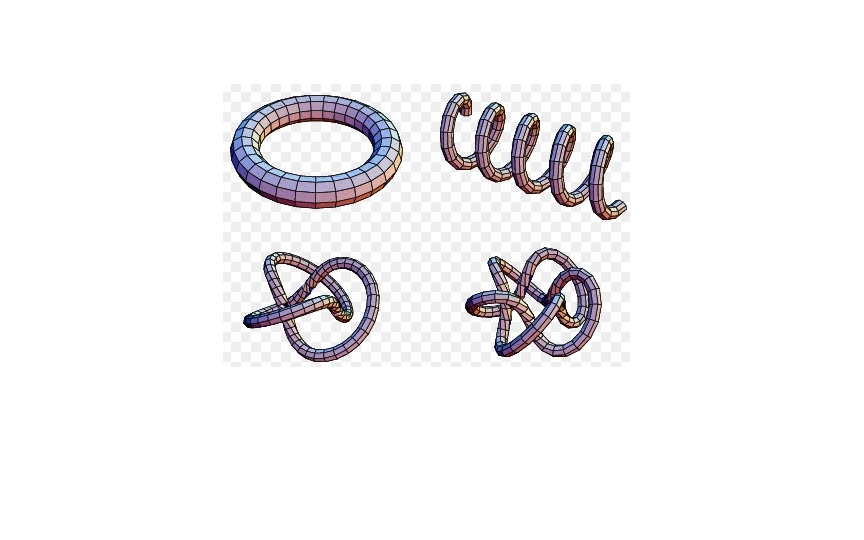
\includegraphics[width=\textwidth]{tubes.jpg}

A primeira das quatro figuras, em que um tubo é construído ao redor de um círculo e que lembra a forma do doce \textit{donut}, é chamada de  \textit{Toro}.

\newpage

\subsection*{Definição Formal}

Ao longo de todo o curso usamos o livro \textit{Apontamentos de Geometria Diferencial} do português Jorge Picado. Nesta obra, o autor define os tubos da seguinte forma:

Seja:  $\gamma : (\alpha ,\beta) \rightarrow \Re^3$ uma  curva  parametrizada  por  comprimento  de  arco,  para  a qual existe um raio r>0 tal que $k(s)< r^{-1}$para qualquer s $ \epsilon  (\alpha ,\beta)$.  A circunferência
\[ \theta \rightarrow cos\theta N(s) + sin\theta B(s) \]está no plano normal à curva em $\gamma(s)$, plano este perpendicular a tangente à curva em $\gamma(s)$.  Quando esta circunferência se move ao longo de $\gamma$ define uma superfície, chamada tubo de raio $r>0$ em torno de $\gamma$, parametrizada por
\[\sigma(s,\theta) =\gamma(s) +r(cos\theta N(s) + sin\theta B(s));\]

com s $\epsilon (\alpha ;\beta), \theta \epsilon  (0,2\pi)$ ou $s \epsilon (\alpha, \beta), \theta (-\pi,\pi)$.

\subsection*{Implementação computacional da função tubo}

Implementamos a definição matemática acima em Matlab com o seguinte código: 

\lstinputlisting{tubo.m}

Há de ser ressaltado que essa função não é um caso particular e sim uma implementação geral. Dessa forma, ela funciona para qualquer curva parametrizada por comprimento de arco.

\subsection*{Exemplos}

No caso do toro temos:

\lstinputlisting{toro.m}

\begin{figure}[h!]
  \caption{}
  \centering
  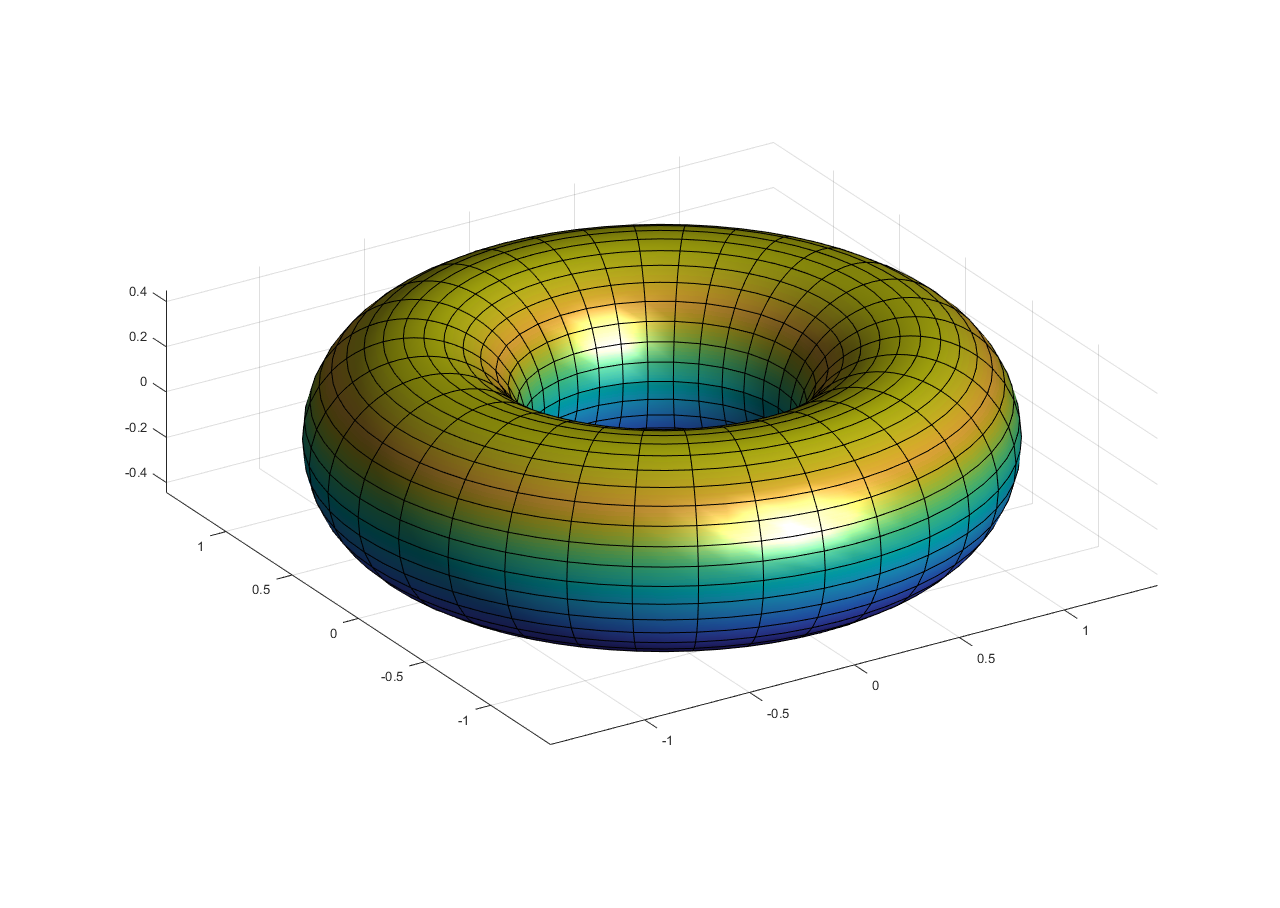
\includegraphics[width=0.75\textwidth]{toro.png}
\end{figure}

\newpage

Outro exemplo interessante é o caso do tubo em formato de espiral. Este pode ser construído da seguinte forma: 

\lstinputlisting{espeiral.m}


\begin{figure}[h!]
  \caption{}
  \centering
  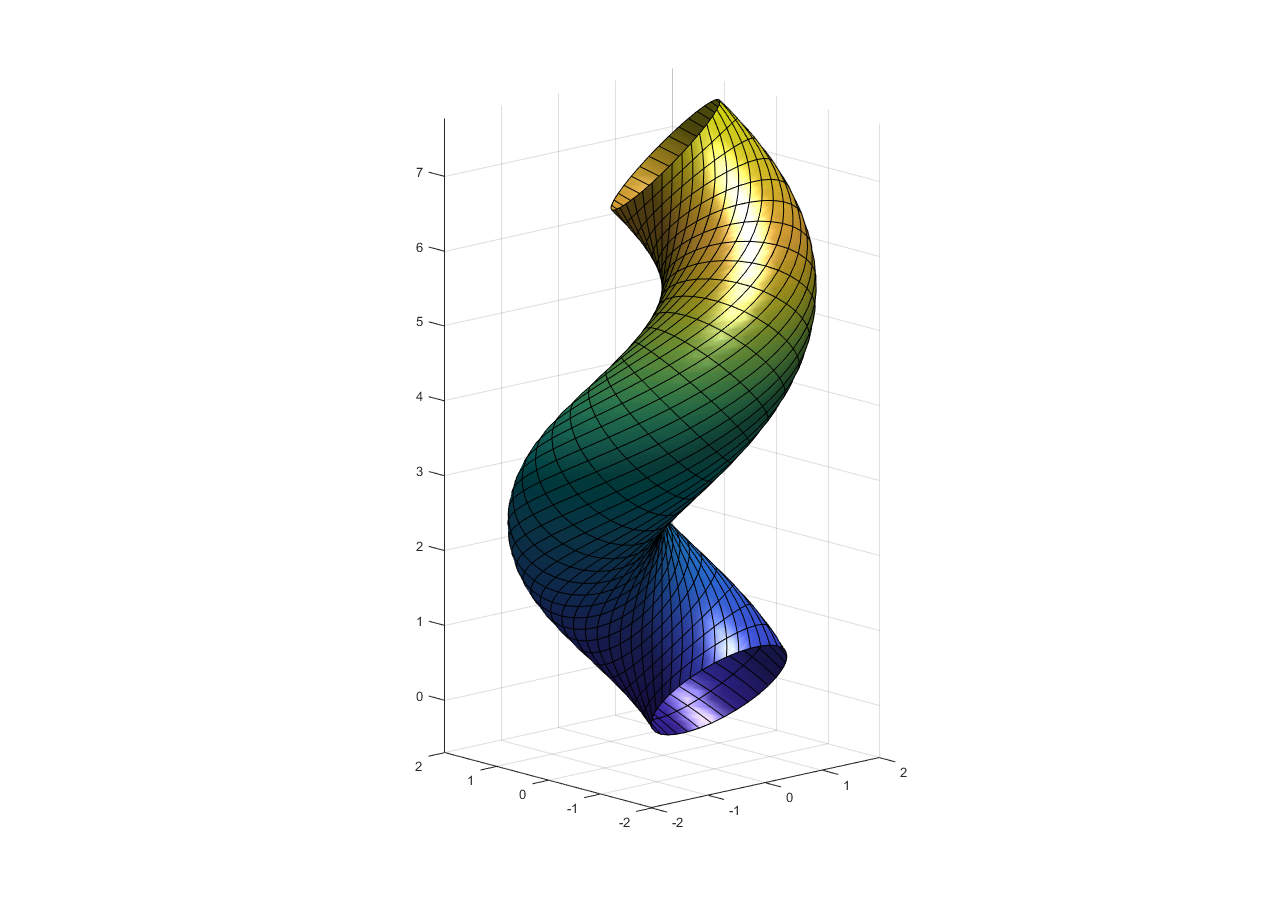
\includegraphics[width=1\textwidth]{espiral.png}
\end{figure}


\newpage

Por fim, cabe citar a implementação com dois tubos em formato de espiral e que possuem raios distintos:

\lstinputlisting{doistubos.m}


\begin{figure}[h!]
  \caption{}
  \centering
  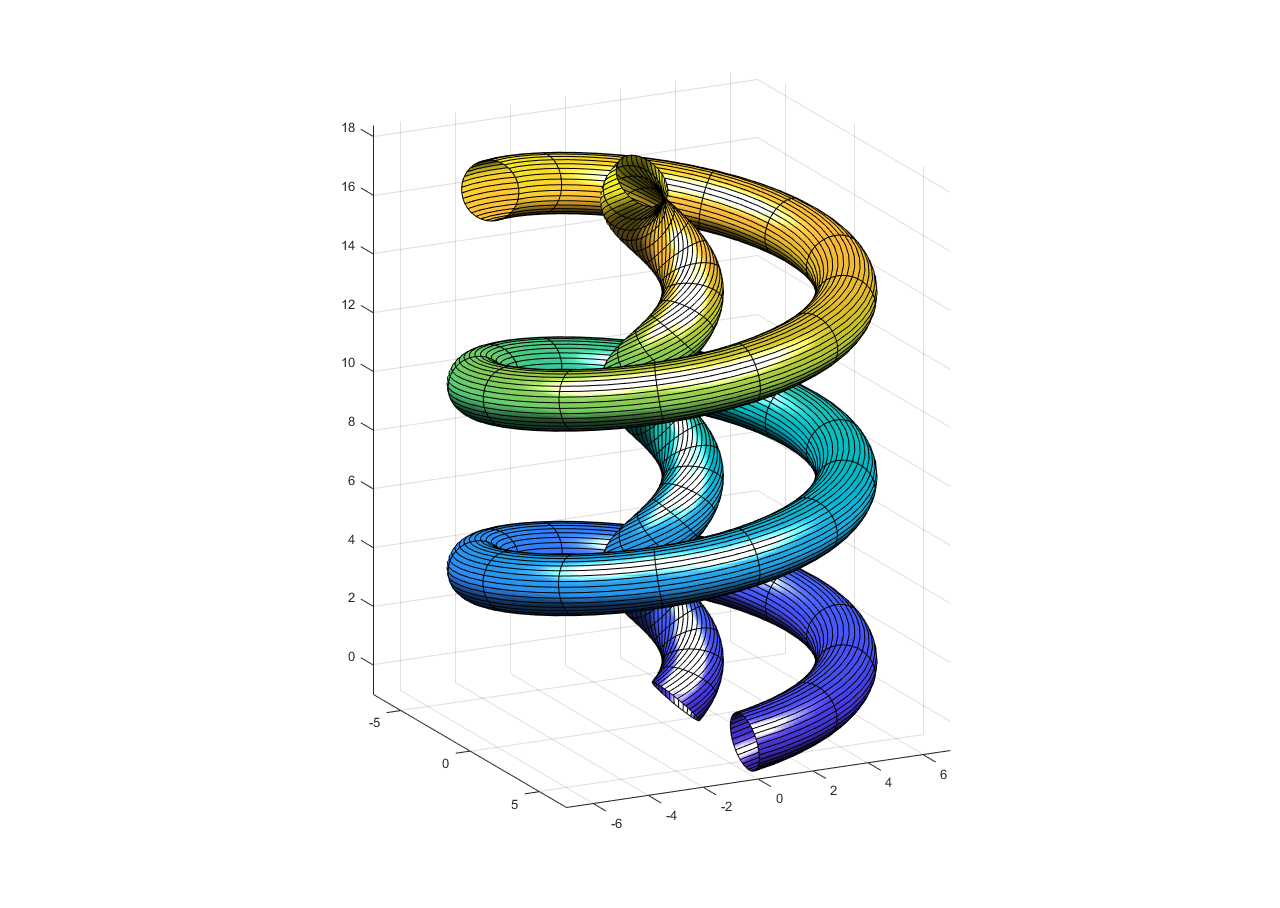
\includegraphics[width=1\textwidth]{doistubos.png}
\end{figure}

\newpage

\subsection{Conchas (Bibi e Fernanda)}
As conchas são um caso particular dos tubos. Ambas as superfícies são geradas a partir de um círculo ou elipse cujo centro se desloca ao longo de uma curva, porém, no caso de conchas, \textbf{o raio varia ao longo da curva.}

Segundo Picado\footnote{\textit{A beleza matemática das conchas marinhas}. Jorge Picado}, uma concha é resultado do deslocamento de uma curva $C$ de centro $P$ (a curva geratriz, geralmente uma elipse) ao longo de uma espiral helicoidal $H$ (a curva estrutural), onde $P \in H$. A curva $C$ pode ser determinada a partir dos vetores normal, $N$, e binormal, $B$, de $H$ no ponto $P$:

\[ C = P(t) + aNcos(\theta) + bBsin(\theta), \]
onde $\theta$ é o ângulo de rotação de um ponto $Q \in C$ no plano formado pelos eixos da elipse e t é o parâmetro da espiral helicoidal $H$.

Na natureza, podemos observar a manifestação dessas figuras nos moluscos. Essa é uma das características mais marcantes desses animais, servindo para a classificação dos mesmos em subgrupos. Vejamos alguns exemplos:

A partir de uma elipse como curva geratriz $C$, podemos gerar conchas como na figura abaixo. Essa concha, chamada \textit{Planorbis}, também dá nome a uma família de gastrópodes, os \textit{Planorbidae}\footnote{Planorbidae. \textit{Wikipédia, a enciclopédia livre.}}.

\begin{figure}[h!]
\centering
\begin{subfigure}{.5\textwidth}
  \centering
  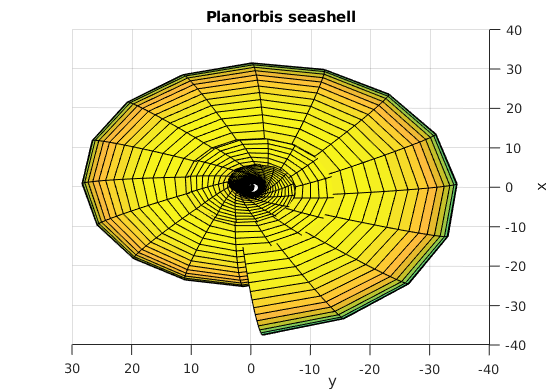
\includegraphics[width=.9\textwidth]{planorbis_up.png}
  \caption{Vista aérea}
  \label{planorbis_up}
\end{subfigure}%
\begin{subfigure}{.5\textwidth}
  \centering
  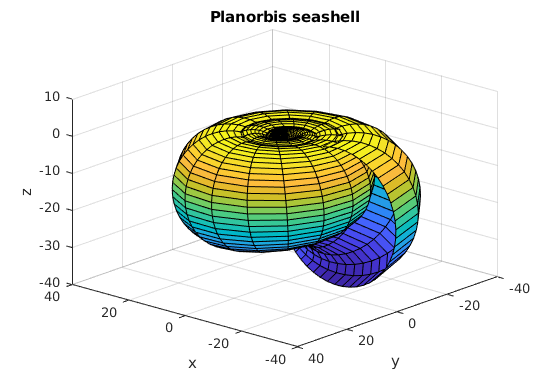
\includegraphics[width=.9\textwidth]{planorbis_front.png}
  \caption{Vista frontal}
  \label{fig:sub2}
\end{subfigure}
\caption{Concha Planorbis (fóssil)}
\label{planorbis_front}
\end{figure}

\lstinputlisting{planorbis.m}
\hfill \\

Um outro tipo de concha pode ser encontrada em moluscos da classe \textit{Bivalve}, que dão o nome à concha\footnote{Bivalvia. \textit{Wikipédia, a enciclopédia livre.}}. Ela é constituída de duas partes iguais, um exemplo de formato de cada uma das partes é o da figura abaixo. Neste caso, a curva geratriz $C$ é uma circunferência, cujo raio varia ao longo de $H$.

\begin{figure}[h!]
\centering
\begin{subfigure}{.5\textwidth}
  \centering
  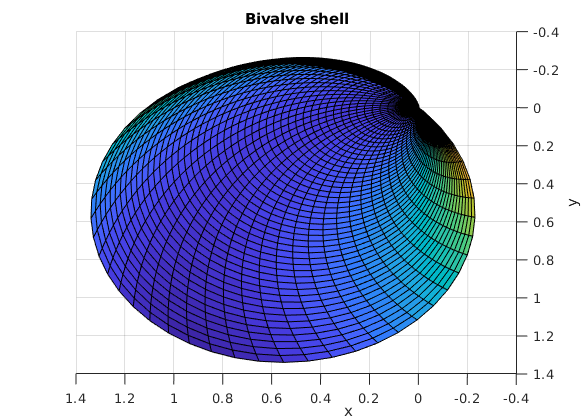
\includegraphics[width=.9\textwidth]{bivalve_up.png}
  \caption{Vista aérea}
  \label{planorbis_up}
\end{subfigure}%
\begin{subfigure}{.5\textwidth}
  \centering
  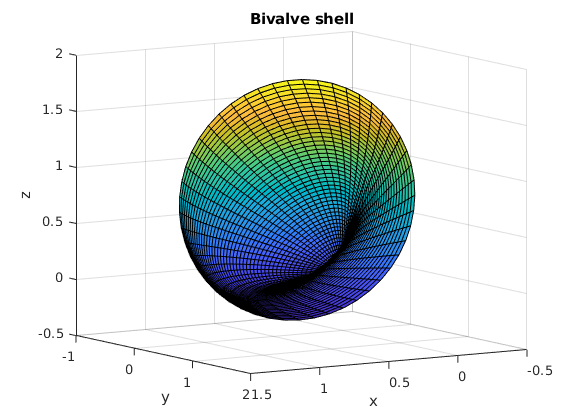
\includegraphics[width=.9\textwidth]{bivalve_front.png}
  \caption{Vista frontal}
  \label{fig:sub2}
\end{subfigure}
\caption{Concha Bivalve}
\label{planorbis_front}
\end{figure}

\lstinputlisting{bivalve.m}
\hfill \\
O formato de $C$ e $H$ nos permite gerar os mais variados tipos de conchas. Alguns exemplos do Picado\footnote{\textit{A beleza matemática das conchas marinhas}. Jorge Picado}, utilizando também rotações da elipse $C$ em torno de seus próprios eixos, ilustram essa diversidade.

\begin{figure}[h!]
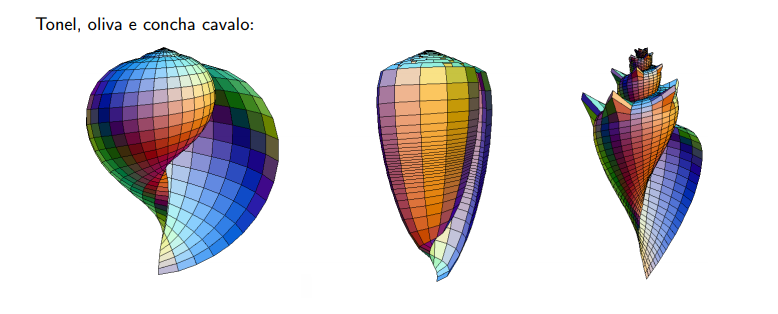
\includegraphics[width=.9\textwidth]{picado_conchas.png}
  \caption{Outros exemplos de conchas}
  \label{picado_conchas}
\end{figure}

\subsection{Superfícies Regradas (Paula e Carla, Fifi)}
Uma superfície regrada $S$ é uma superfície que em cada ponto $p ∈ S$, existe um segmento de reta contido em $S$ passando por $p$. 
\\
\textbf{Observação:} Uma forma de obter superfícies regradas é tomar uma parametrização da forma $f(u,v)=g(u)+v.h(u)$, onde $g$ e $h$ são curvas diferenciáveis.
\\
\begin{enumerate}
\item A função $f(u,v)=(cos(u),sin(u),1)+v(0,0,1)$ define uma superfície regrada.
\lstinputlisting{braceletecod.m}
\begin{figure}[H]
\centering
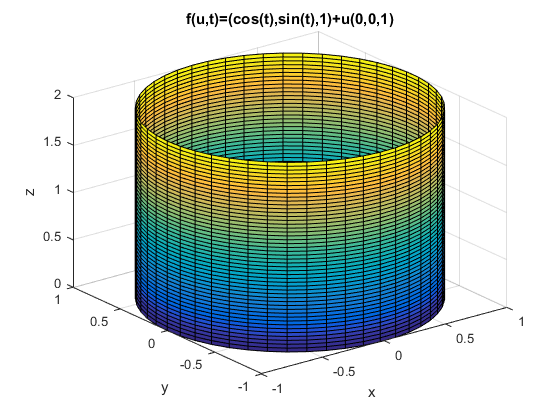
\includegraphics[height=10cm]{bracelete.png}
\caption{Superfície similar a um bracelete}
\label{gráfico1}
\end{figure}
\item O helicóide definido por $f(u,v)=g(u)+v.h(u)$ onde $g(u)=(acos(u),asin(u),u)$ e $h(u)=(−cos(u),-sin(u),0)$, é uma superfície regrada.
\lstinputlisting{helicoidecod.m}
\begin{figure}[H]
\centering
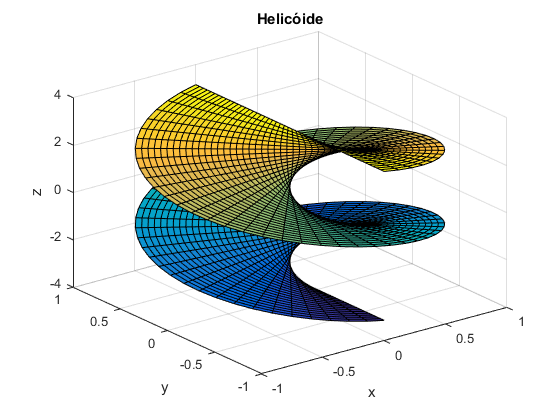
\includegraphics[height=11cm]{Helicoide_imagem.png}
\caption{Helicóide}
\label{gráfico2}
\end{figure}
\item Outra superfície regrada conhecida é a superfície obtida a partir da curva de Viviani. Em Matemática, particularmente Geometria, a curva de Viviani, também conhecida como janela de Viviani, é uma curva no espaço figura em forma de oito nomeada em homenagem ao matemático italiano Vincenzo Viviani, a intersecção de uma esfera com um cilindro que é tangente à esfera e passa através do centro da esfera.
\begin{figure}[H]
\centering
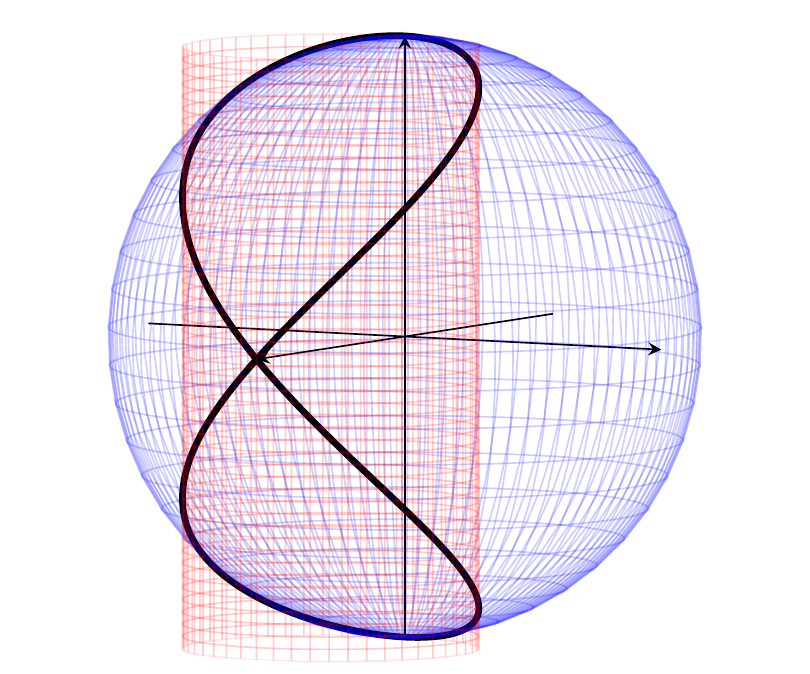
\includegraphics[height=8cm]{vick.png}
\caption{Curva de Viviani}
\label{gráfico3}
\end{figure}
A parametrização da superfície é dada pela seguinte equação:
\\
$$f(u,t)=(1+cos(t),sin(t),2sin(\frac{t}{2}))+u(-sin(t),cos(t),cos(\frac{t}{2}))$$
\lstinputlisting{curva_vivi.m}
\begin{figure}[H]
\centering
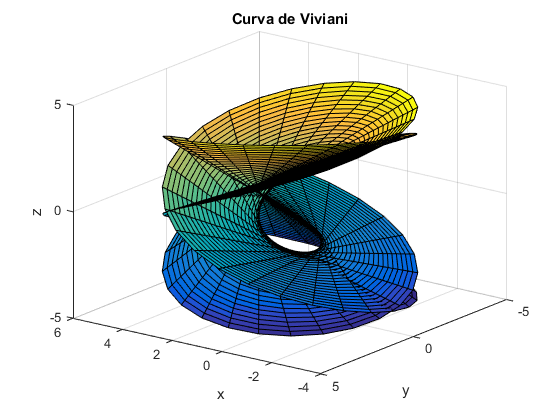
\includegraphics[height=11cm]{Curva_de_Viviani.png}
\caption{Curva de Viviani}
\label{gráfico4}
\end{figure}
\item O guarda-chuva Whitney (às vezes chamado de guarda-chuva Cayley) é uma superfície auto-intersectada colocada em três dimensões.É a união de todas as linhas retas que passam por pontos de uma parábola fixa e são perpendiculares a uma linha reta fixa, paralelamente ao eixo da parábola e deitada no seu plano de divisão perpendicular (bisecção/bissetriz). A parametrização é dada por:
$$f(u,t)=(t^2,0,0)+u(0,\frac{1}{\sqrt{1+t^2}},\frac{t}{\sqrt{1+t^2}})$$
\lstinputlisting{guarda_chuva.m}
\begin{figure}[H]
\centering
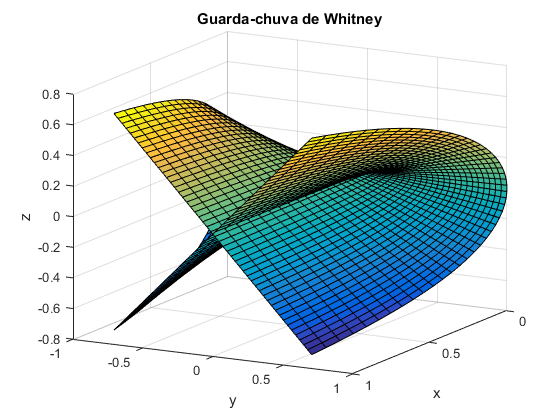
\includegraphics[height=11cm]{Guarda_chuva_de_Whitney.png}
\caption{Guarda-chuva de Whitney}
\label{gráfico5}
\end{figure}
\end{enumerate}
\subsection{Superfícies de Revolução (Rafael Katz, Rafael Paya e Emerson Lai)}
Uma superfície de revolução é uma superfície gerada por uma rotação de uma curva plana ou cônica, chamada geratriz, em torno de um dos eixos ou em torno de uma reta fixa nesse plano, chamado de eixo de revolução.Por exemplo, a esfera e o toro são superfcies de revolucão representado nas imagens abaixo. 

\begin{figure}[h!]
  \caption{Esfera}
  \centering
  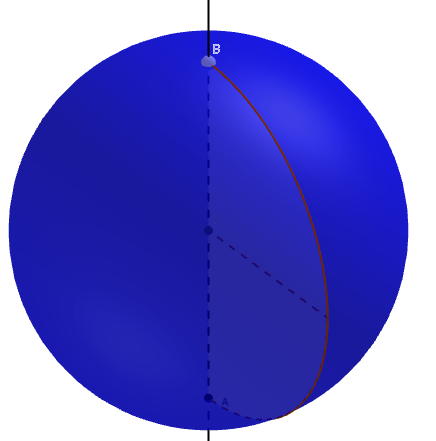
\includegraphics[width=0.5\textwidth]{cone_revolucao.png}
\end{figure}

\begin{figure}[h!]
  \caption{Toro}
  \centering
  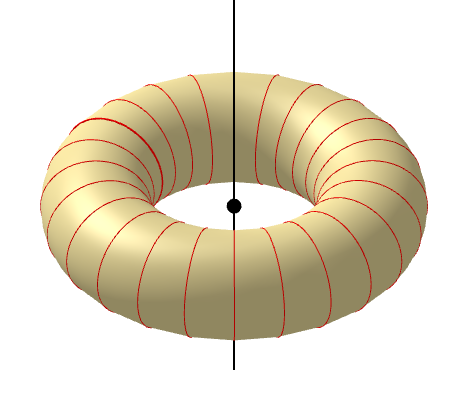
\includegraphics[width=0.5\textwidth]{toro_revolucao.png}
\end{figure}

\section*{Construção dessas figuras usando Matlab} 
\subsection*{Esfera}
\lstset{language=matlab}

\begin{lstlisting}[frame=single]
syms u v;
a = 1;
figure(1);
alpha1 = [a*cos(u)*sin(v),a*sin(u)*sin(v),a*cos(v)];
ezsurf(alpha1(1),alpha1(2),alpha1(3),[0,2*pi,0.01,pi]);
axis([-1 1 -1 1]);
for k = 0:0.1:2
    alpha1 = [a*cos(u)*sin(v),a*sin(u)*sin(v),a*cos(v)];
    ezsurf(alpha1(1),alpha1(2),alpha1(3),[0,k*pi,0.01,pi]);
    axis([-1 1 -1 1]);
    pause(0.05);
end
\end{lstlisting}
\subsection*{toro}
\begin{lstlisting}[frame=single]
syms u v;
R = 3;
r = 2;
colormap spring;
figure(1);
alpha1 = [(R+r*cos(u))*cos(v),r*sin(u),(R+r*cos(u))*sin(v),r*sin(u)];
ezsurf(alpha1(1),alpha1(2),alpha1(3),[0,2*pi,0.01,2*pi]);

axis([-5,5,-5,5,-5,5])


for k = 0:0.1:2
    alpha1 = [(R+r*cos(u))*cos(v),(R+r*cos(u))*sin(v),r*sin(u)];
    ezsurf(alpha1(1),alpha1(2),alpha1(3),[0,k*pi,0.01,2*pi]);
    axis([-5,5,-5,5,-5,5]);
    pause(0.05);
end
\end{lstlisting}
\subsection*{Cone Duplo}
\begin{lstlisting}[frame=single]
syms u v;
h = 3;
r = 2;
colormap spring;
figure(1);
alpha1 = [(h-v)/h*r*cos(u),(h-v)/h*r*sin(u),v];
ezsurf(alpha1(1),alpha1(2),alpha1(3),[0,2*pi,0.01,2*pi]);

axis([-5,5,-5,5,-5,5])


for k = 0:0.1:2
    alpha1 = [(h-v)/h*r*cos(u),(h-v)/h*r*sin(u),v];
    ezsurf(alpha1(1),alpha1(2),alpha1(3),[0,k*pi,0.01,2*pi]);
    axis([-5,5,-5,5,-5,5]);
    pause(0.05);
end
\end{lstlisting}
\subsection*{Gabriel's Horn}
Trombeta de Gabriel, é uma superfície de revolução que se obtém girando a curva ${ y=x^{-1}}$ , com ${ x\in [1,\infty )}$ , em torno do eixo das abscissas. Tal construção tem a característica de possuir uma superfície com área infinita, envolvendo um volume finito.

\begin{figure}[h!]
  \caption{trompeta de gabriel}
  \centering
  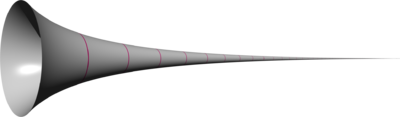
\includegraphics[width=0.5\textwidth]{trompeta_de_gabriel.png}
\end{figure}

\begin{lstlisting}[frame=single]
syms u v;
a = 3;
colormap spring;
figure(1);
alpha1 = [u,a*cos(v)/u,a*sin(v)/u];
ezsurf(alpha1(1),alpha1(2),alpha1(3),[0,2*pi,0.01,2*pi]);

axis([-5,5,-5,5,-5,5])


for k = 0:0.1:2
    alpha1 = [u,a*cos(v)/u,a*sin(v)/u];
    ezsurf(alpha1(1),alpha1(2),alpha1(3),[0,k*pi,0.01,2*pi]);
    axis([-5,5,-5,5,-5,5]);
    pause(0.05);
end

\end{lstlisting}

\section{Comentários e bibliografia \LaTeX{}}

Como colocar comentários (útil para o ambiente colaborativo do overleaf):

Comments can be added to your project by clicking on the comment icon in the toolbar above. % * <john.hammersley@gmail.com> 2014-09-03T09:54:16.211Z:
%
% Here's an example comment!
%
To reply to a comment, simply click the reply button in the lower right corner of the comment, and you can close them when you're done.

You can upload a \verb|.bib| file containing your BibTeX entries, created with JabRef; or import your \href{https://www.overleaf.com/blog/184}{Mendeley}, CiteULike or Zotero library as a \verb|.bib| file. You can then cite entries from it, like this: \cite{greenwade93}. Just remember to specify a bibliography style, as well as the filename of the \verb|.bib|.

You can find a \href{https://www.overleaf.com/help/97-how-to-include-a-bibliography-using-bibtex}{video tutorial here} to learn more about BibTeX.

We hope you find Overleaf useful, and please let us know if you have any feedback using the help menu above --- or use the contact form at \url{https://www.overleaf.com/contact}!

\bibliographystyle{alpha}
\bibliography{sample}

\end{document}